\documentclass{article}
\usepackage{tikz}
\usetikzlibrary{arrows.meta, positioning, calc}

\begin{document}

\section*{Figure 1: Diagnostic Medicine Scenario}
% W1, W2: illnesses
% X: toxin-lowering treatment
% Y1, Y2: survival
% Dashed bidirected edges: hidden confounding factors

\subsection*{(a) Effect is Identifiable}
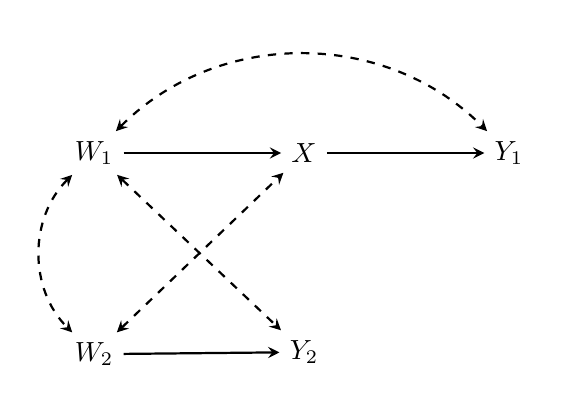
\begin{tikzpicture}[>=stealth, node distance=2cm and 2cm, thick]
    % Nodes
    \node (W1) {$W_1$};
    \node (X) [right=of W1] {$X$};
    \node (Y1) [right=of X] {$Y_1$};
    \node (W2) [below=of W1] {$W_2$};
    \node (Y2) [below=of X] {$Y_2$};

    % Directed edges (causal mechanisms)
    \draw[->] (W1) -- (X);
    \draw[->] (X) -- (Y1);
    \draw[->] (W2) -- (Y2);
    
    % Bidirected edges (hidden confounders)
    \draw[<->, dashed, bend left=45] (W1) to (Y1);
    \draw[<->, dashed, bend right=45] (W1) to (W2);
    \draw[<->, dashed] (W2) to (X);
    \draw[<->, dashed] (W1) to (Y2);
\end{tikzpicture}

\subsection*{(b) Effect is NOT Identifiable (Hedge Structure)}
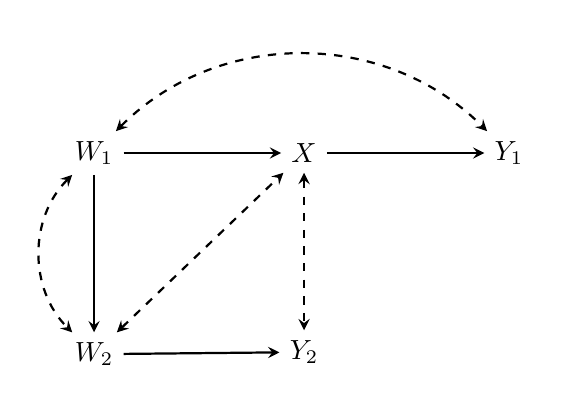
\begin{tikzpicture}[>=stealth, node distance=2cm and 2cm, thick]
    % Nodes
    \node (W1) {$W_1$};
    \node (X) [right=of W1] {$X$};
    \node (Y1) [right=of X] {$Y_1$};
    \node (W2) [below=of W1] {$W_2$};
    \node (Y2) [below=of X] {$Y_2$};

    % Directed edges (causal mechanisms)
    \draw[->] (W1) -- (X);
    \draw[->] (X) -- (Y1);
    \draw[->] (W1) -- (W2); % Added causal link forming part of the hedge
    \draw[->] (W2) -- (Y2);
    
    % Bidirected edges (hidden confounders)
    \draw[<->, dashed, bend left=45] (W1) to (Y1);
    \draw[<->, dashed, bend right=45] (W1) to (W2);
    \draw[<->, dashed] (W2) to (X);
    \draw[<->, dashed] (X) to (Y2);
\end{tikzpicture}

\vspace{1cm}
\documentclass{article}
\usepackage{tikz}
\usetikzlibrary{arrows.meta, positioning, calc}

\begin{document}

\section*{Figure 1: Diagnostic Medicine Scenario}
% W1, W2: illnesses
% X: toxin-lowering treatment
% Y1, Y2: survival
% Dashed bidirected edges: hidden confounding factors

\subsection*{(a) Effect is Identifiable}
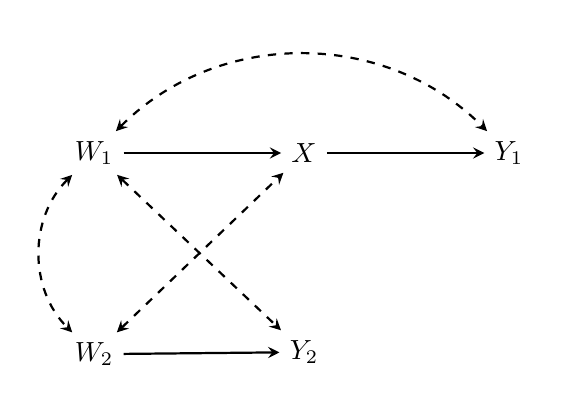
\begin{tikzpicture}[>=stealth, node distance=2cm and 2cm, thick]
    % Nodes
    \node (W1) {$W_1$};
    \node (X) [right=of W1] {$X$};
    \node (Y1) [right=of X] {$Y_1$};
    \node (W2) [below=of W1] {$W_2$};
    \node (Y2) [below=of X] {$Y_2$};

    % Directed edges (causal mechanisms)
    \draw[->] (W1) -- (X);
    \draw[->] (X) -- (Y1);
    \draw[->] (W2) -- (Y2);
    
    % Bidirected edges (hidden confounders)
    \draw[<->, dashed, bend left=45] (W1) to (Y1);
    \draw[<->, dashed, bend right=45] (W1) to (W2);
    \draw[<->, dashed] (W2) to (X);
    \draw[<->, dashed] (W1) to (Y2);
\end{tikzpicture}

\subsection*{(b) Effect is NOT Identifiable (Hedge Structure)}
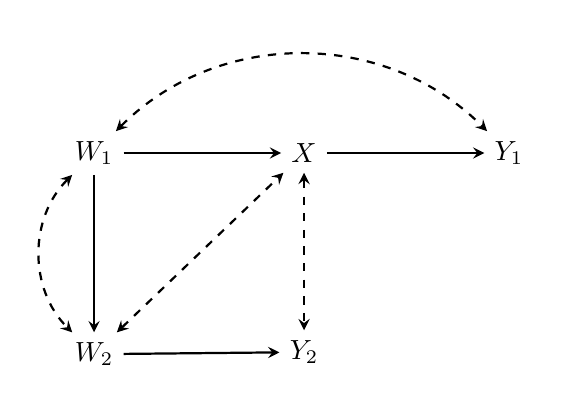
\begin{tikzpicture}[>=stealth, node distance=2cm and 2cm, thick]
    % Nodes
    \node (W1) {$W_1$};
    \node (X) [right=of W1] {$X$};
    \node (Y1) [right=of X] {$Y_1$};
    \node (W2) [below=of W1] {$W_2$};
    \node (Y2) [below=of X] {$Y_2$};

    % Directed edges (causal mechanisms)
    \draw[->] (W1) -- (X);
    \draw[->] (X) -- (Y1);
    \draw[->] (W1) -- (W2); % Added causal link forming part of the hedge
    \draw[->] (W2) -- (Y2);
    
    % Bidirected edges (hidden confounders)
    \draw[<->, dashed, bend left=45] (W1) to (Y1);
    \draw[<->, dashed, bend right=45] (W1) to (W2);
    \draw[<->, dashed] (W2) to (X);
    \draw[<->, dashed] (X) to (Y2);
\end{tikzpicture}

\vspace{1cm}
\section*{Figure 2: Graphs where $P_x(Y)$ is not identifiable}
% Nodes are arranged to match the structural constraints defined in the paper:
% - Y-rooted C-trees (d, e, f, h) must have every observable with at most one child, 
%   and their bidirected edges must form a spanning tree.
% - Graphs (b, c) have two C-components {X,Z} and {Y}.
% - Graph (g) is the classic unidentifiable kite/w-graph structure.

\vspace{0.5cm}

\begin{tikzpicture}[>=stealth, thick]

    % -------------------------------------------------------------
    % (a) The Bow Arc Graph
    % -------------------------------------------------------------
    \begin{scope}[local bounding box=A]
        \node (X) {$X$};
        \node (Y) [below=1.5cm of X] {$Y$};
        
        \draw[->] (X) -- (Y);
        \draw[<->, dashed, bend left=60] (X) to (Y);
        \node[below=0.5cm of Y] {(a)};
    \end{scope}

    % -------------------------------------------------------------
    % (b) X->Z->Y with X<->Z
    % Two C-components: {X,Z} and {Y}
    % -------------------------------------------------------------
    \begin{scope}[xshift=4cm, local bounding box=B]
        \node (X) {$X$};
        \node (Z) [below right=0.75cm and 0.75cm of X] {$Z$};
        \node (Y) [below left=0.75cm and 0.75cm of Z] {$Y$};
        
        \draw[->] (X) -- (Z);
        \draw[->] (Z) -- (Y);
        \draw[<->, dashed, bend left=45] (X) to (Z);
        \node[below=0.5cm of Y] {(b)};
    \end{scope}

    % -------------------------------------------------------------
    % (c) X->Z->Y with X->Y and X<->Z
    % Two C-components: {X,Z} and {Y}
    % -------------------------------------------------------------
    \begin{scope}[xshift=8cm, local bounding box=C]
        \node (X) {$X$};
        \node (Z) [below right=0.75cm and 0.75cm of X] {$Z$};
        \node (Y) [below left=0.75cm and 0.75cm of Z] {$Y$};
        
        \draw[->] (X) -- (Z);
        \draw[->] (Z) -- (Y);
        \draw[->] (X) -- (Y);
        \draw[<->, dashed, bend left=45] (X) to (Z);
        \node[below=0.5cm of Y] {(c)};
    \end{scope}

    % -------------------------------------------------------------
    % (d) Y-rooted C-tree (X->Y, Z->Y)
    % -------------------------------------------------------------
    \begin{scope}[yshift=-5cm, local bounding box=D]
        \node (X) {$X$};
        \node (Z) [right=1.5cm of X] {$Z$};
        \node (Y) [below right=1.5cm and 0.75cm of X] {$Y$};
        
        \draw[->] (X) -- (Y);
        \draw[->] (Z) -- (Y);
        % Bidirected spanning tree
        \draw[<->, dashed, bend left=45] (X) to (Z);
        \draw[<->, dashed, bend left=45] (Z) to (Y);
        \node[below=0.5cm of Y] {(d)};
    \end{scope}

    % -------------------------------------------------------------
    % (e) Y-rooted C-tree (X->Z->Y variant 1)
    % -------------------------------------------------------------
    \begin{scope}[xshift=4cm, yshift=-5cm, local bounding box=E]
        \node (X) {$X$};
        \node (Z) [below=1cm of X] {$Z$};
        \node (Y) [below=1cm of Z] {$Y$};
        
        \draw[->] (X) -- (Z);
        \draw[->] (Z) -- (Y);
        % Bidirected spanning tree
        \draw[<->, dashed, bend left=60] (X) to (Z);
        \draw[<->, dashed, bend left=60] (X) to (Y);
        \node[below=0.5cm of Y] {(e)};
    \end{scope}

    % -------------------------------------------------------------
    % (f) Y-rooted C-tree (X->Z->Y variant 2)
    % -------------------------------------------------------------
    \begin{scope}[xshift=8cm, yshift=-5cm, local bounding box=F]
        \node (X) {$X$};
        \node (Z) [below=1cm of X] {$Z$};
        \node (Y) [below=1cm of Z] {$Y$};
        
        \draw[->] (X) -- (Z);
        \draw[->] (Z) -- (Y);
        % Bidirected spanning tree
        \draw[<->, dashed, bend left=60] (Z) to (Y);
        \draw[<->, dashed, bend left=60] (X) to (Y);
        \node[below=0.5cm of Y] {(f)};
    \end{scope}

    % -------------------------------------------------------------
    % (g) The "Kite" Structure (X->Z1, X->Z2, Z1->Y, Z2->Y)
    % -------------------------------------------------------------
    \begin{scope}[yshift=-11cm, xshift=2cm, local bounding box=G]
        \node (X) {$X$};
        \node (Z1) [below left=1cm and 1cm of X] {$Z_1$};
        \node (Z2) [below right=1cm and 1cm of X] {$Z_2$};
        \node (Y) [below right=1cm and 1cm of Z1] {$Y$};
        
        \draw[->] (X) -- (Z1);
        \draw[->] (X) -- (Z2);
        \draw[->] (Z1) -- (Y);
        \draw[->] (Z2) -- (Y);
        % Hedge confounders
        \draw[<->, dashed] (Z1) to (Z2);
        \draw[<->, dashed, bend right=45] (Z1) to (Y);
        \node[below=0.5cm of Y] {(g)};
    \end{scope}

    % -------------------------------------------------------------
    % (h) 4-node Y-rooted C-tree (Z->X->W->Y)
    % -------------------------------------------------------------
    \begin{scope}[yshift=-11cm, xshift=7cm, local bounding box=H]
        \node (Z) {$Z$};
        \node (X) [right=1cm of Z] {$X$};
        \node (W) [right=1cm of X] {$W$};
        \node (Y) [right=1cm of W] {$Y$};
        
        \draw[->] (Z) -- (X);
        \draw[->] (X) -- (W);
        \draw[->] (W) -- (Y);
        % Bidirected spanning tree over all 4 nodes
        \draw[<->, dashed, bend left=45] (Z) to (W);
        \draw[<->, dashed, bend right=45] (X) to (Y);
        \draw[<->, dashed, bend left=45] (Z) to (X);
        
        \node[below=1.5cm of X, xshift=0.5cm] {(h)};
    \end{scope}

\end{tikzpicture}

\end{document}

\section*{Figure 2: Examples of Unidentifiable Graphs}

\subsection*{(a) The Classic "Bow Arc" Graph}
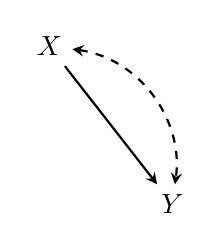
\begin{tikzpicture}[>=stealth, node distance=2cm, thick]
    % Nodes
    \node (X) {$X$};
    \node (Y) [below right=1.5cm and 1cm of X] {$Y$};

    % Directed edge
    \draw[->] (X) -- (Y);
    
    % Bidirected edge
    \draw[<->, dashed, bend left=45] (X) to (Y);
\end{tikzpicture}

\subsection*{(b) Y-Rooted C-Tree}
\begin{tikzpicture}[>=stealth, node distance=1.5cm, thick]
    % Nodes
    \node (X) {$X$};
    \node (Z) [below right=of X] {$Z$};
    \node (Y) [below=of Z] {$Y$};

    % Directed edges
    \draw[->] (X) -- (Z);
    \draw[->] (Z) -- (Y);
    
    % Bidirected edges
    \draw[<->, dashed, bend left=45] (X) to (Z);
\end{tikzpicture}

\subsection*{(c) C-Component causing non-identifiability}
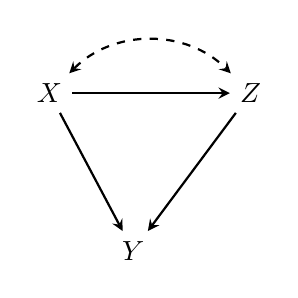
\begin{tikzpicture}[>=stealth, node distance=2cm, thick]
    % Nodes
    \node (X) {$X$};
    \node (Z) [right=of X] {$Z$};
    \node (Y) [below right=1.5cm and 0.5cm of X] {$Y$};

    % Directed edges
    \draw[->] (X) -- (Y);
    \draw[->] (X) -- (Z);
    \draw[->] (Z) -- (Y);
    
    % Bidirected edges
    \draw[<->, dashed, bend left=45] (X) to (Z);
\end{tikzpicture}

\end{document}
\end{document}